\chapter{Background Estimate }

\section{Monte Carlo }
{\normalsize - MC's used, PDF's, k-factors}
\newpage
\section{Fake Factor Multi-Jet Estimate }

One of the major sources of background to di-electron signals are di-jets or electron+jets (mainly W+jets) events where one or both selected leptons are jets faking electron signatures. The method for estimating this background, described here, is a "fake factor" or "matrix-method". This is a data-driven method where electrons are selected by a tight ($N_{tight}$) and loose ($N_{loose}$) selection. The tight selection is the standard electron selection used in this analysis while the loose selection has no isolation requirement and must only pass a loose++ egamma definition (see Chapter 4) with no track matching criteria. $N_{tight}$ is therefore by design a subset of $N_{loose}$. Two more hidden values are also assigned $real$ and $fake$ referring to true source of each electron. This gives us two coefficients to determine from data.

\begin{equation} \label{eq:fakeRate}
   f~=~\frac{N^{fake}_{tight}}{N^{fake}_{loose}} \qquad \qquad r~=~\frac{N^{real}_{tight}}{N^{real}_{loose}}
\end{equation}

The fake rate $f$ denotes the probability that a $fake$ electron which passes the loose requirement also passes tight while $r$ refers to the probability that a $real$ electron which passes the loose requirement also passes the tight.
Reconstructed events are split in to two distinct groups, tight($T$), and loose while failing tight($L$), where $Tight$ is now no longer a subset of $Loose$. This allows us to relate our reconstructed events to the underling truth events via a matrix of fake rates shown in Eq.~\ref{eq:mainFakeMatrix}.

\begin{equation} \label{eq:mainFakeMatrix}
   \begin{pmatrix}
      N_{TT} \\
      N_{TL} \\
      N_{LT} \\
      N_{LL} \\
   \end{pmatrix}
   =
   \begin{pmatrix}
      r_{1}r_{2} & r_{1}f_{2} & f_{1}r_{2} & f_{1}f_{2} \\
      r_{1}(1-r_{2}) & r_{1}(1-f_{2}) & f_{1}(1-r_{2}) & f_{1}(1-f_{2}) \\
      (1-r_{1})r_{2} & (1-r_{1})f_{2} & (1-f_{1})r_{2} & (1-f_{1})f_{2} \\
      (1-r_{1})(1-r_{2}) & (1-r_{1})(1-f_{2}) & (1-f_{1})(1-r_{2}) & (1-f_{1})(1-f_{2}) \\
   \end{pmatrix}
   \begin{pmatrix}
      N_{RR} \\
      N_{RF} \\
      N_{FR} \\
      N_{FF} \\
   \end{pmatrix}
\end{equation}

The first index in Eq.~\ref{eq:mainFakeMatrix} refers to the highest $p_{T}$ electron while the second index refers to the second highest $p_{T}$ electron. So $N_{LT}$ indicates the reconstructed events with highest $p_{T}$ electron only passing the $Loose$ selection while the second highest $p_{T}$ electron passes $Tight$ selection. The indices 1 and 2 refer to fake rates ($f$) and efficiencies ($r$) on leading and sub-leading electrons respectively.

The interesting part for this study is the contribution to $N_{TT}$ coming from sources other than $N_{RR}$, these can be seen in Eq.~\ref{eq:multijet}.

\begin{align} \label{eq:multijet}
   N^{\ell+jets}_{TT}~&=~r_{1}f_{2}N_{RF}~+~f_{1}r_{2}N_{FR} \nonumber \\
   N^{di-jets}_{TT}~&=~f_{1}f_{2}N_{FF} \nonumber \\
   N^{\ell+jets~\&~di-jets}_{TT}~&=~r_{1}f_{2}N_{RF}~+~f_{1}r_{2}N_{FR}~+~f_{1}f_{2}N_{FF} 
\end{align}

This function however contains hidden variables and so Eq.~\ref{eq:mainFakeMatrix} is inverted to derive a better formalism.

\begin{equation}
   \begin{pmatrix}
      N_{RR} \\
      N_{RF} \\
      N_{FR} \\
      N_{FF} \\
   \end{pmatrix}
   = \alpha
   \begin{pmatrix}
      (f_{1}-1)(f_{2}-1) & (f_{1}-1)f_{2} & f_{1}(f_{2}-1) & f_{1}f_{2} \\
      (f_{1}-1)(1-r_{2}) & (1-f_{1})r_{2} & f_{1}(1-r_{2}) & -f_{1}r_{2} \\
      (r_{1}-1)(1-f_{2}) & (1-r_{1})f_{2} & r_{1}(1-f_{2}) & -r_{1}f_{2} \\
      (1-r_{1})(1-r_{2}) & (r_{1}-1)r_{2} & r_{1}(r_{2}-1) & r_{1}r_{2} \\
   \end{pmatrix}
   \begin{pmatrix}
      N_{TT} \\
      N_{TL} \\
      N_{LT} \\
      N_{LL} \\
   \end{pmatrix}
\end{equation}

where,

\begin{equation}
   \alpha~=~\frac{1}{(r_{1}-f_{1})(r_{2}-f_{2})}
\end{equation}

The fraction of selected events with at least one fake is then given by Eq.~\ref{eq:mainFakeMatrix}.

\begin{equation}
\begin{aligned}
   N^{\ell+jets~\&~di-jets}_{TT}~&=&~\alpha r_{1}f_{2}[(f_{1}-1)(1-r_{2})N_{TT}~+~(1-f_{1})r_{2}N_{TL}~&+~f_{1}(1-r_{2})N_{LT}~-~f_{1}r_{2}N_{LL}] \\
      &~+&~\alpha f_{1}r_{2}[(r_{1}-1)(1-f_{2})N_{TT}~+~(1-r_{1})f_{2}N_{TL}~&+~r_{1}(1-f_{2})N_{LT}~-~r_{1}f_{2}N_{LL}] \\
      &~+&~\alpha f_{1}f_{2}[(1-r_{1})(1-r_{2})N_{TT}~+~(r_{1}-1)r_{2}N_{TL}~&+~r_{1}(r_{2}-1)N_{LT}~+~r_{1}r_{2}N_{LL}] 
\end{aligned}
\end{equation}

\begin{equation} \label{eq:mainFakeResult}
\begin{aligned}
   =\alpha[r_{1}f_{2}(f_{1}-1)(1-r_{2})~+~f_{1}r_{2}(r_{1}-1)(1-f_{2})~+~f_{1}f_{2}(1-r_{1})(1-r_{2})]N_{TT} \\
   +~\alpha f_{2}r_{2}[r_{1}(1-f_{1})~+~f_{1}(1-r_{1})~+~f_{1}(r_{1}-1)]N_{TL} \\
   +~\alpha f_{1}r_{1}[f_{2}(1-r_{2})~+~r_{2}(1-f_{2})~+~f_{2}(r_{2}-1)]N_{LT} \\
   -~\alpha f_{1}f_{2}r_{1}r_{2}N_{LL}
\end{aligned}
\end{equation}

Equation \ref{eq:mainFakeResult} shows the derived formula relating the multi-jet background to fake rates, efficiencies and four independent samples selected from data. Detailed here is this method used on the full $20~fb^{-1}$ of integrated luminosity from ATLAS's 2012 run.


\subsection{Real electron efficiency estimation}

The real electron efficiency is defined as Eq. ~\ref{eq:fakeRate} $r~=~N^{real}_{tight}/N^{real}_{loose}$. This is determined from MC using a mass binned Drell-Yan sample. The efficiencies are found for both the leading and sub-leading electrons and binned in 8 $p_{T}$ and three eta bins of $|\eta|<1.37$ (barrel), $1.52<|\eta|<2.01$ and $2.01<|\eta|<2.47$ (endcap). The efficiency is distributed between $90$ - $96\%$ as can be seen in Fig. \ref{fig:realEff}.

   \begin{figure}[h]
      \begin{center}
      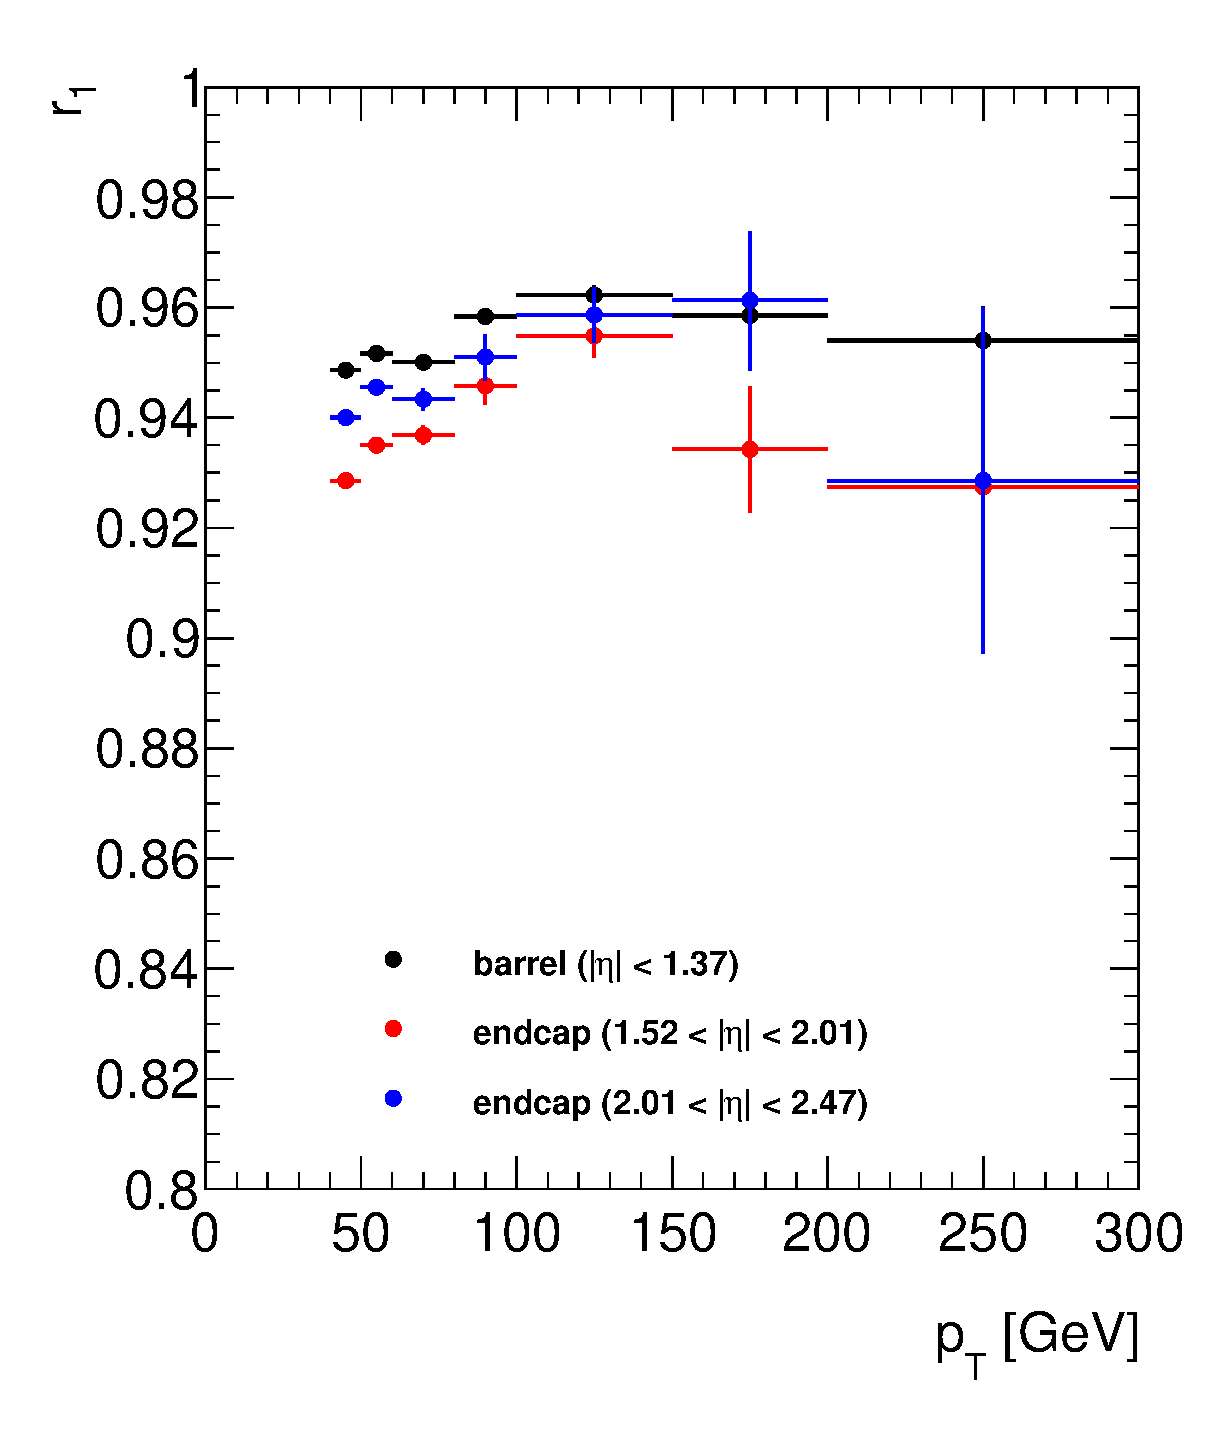
\includegraphics[scale=0.41]{images/r1.eps}
      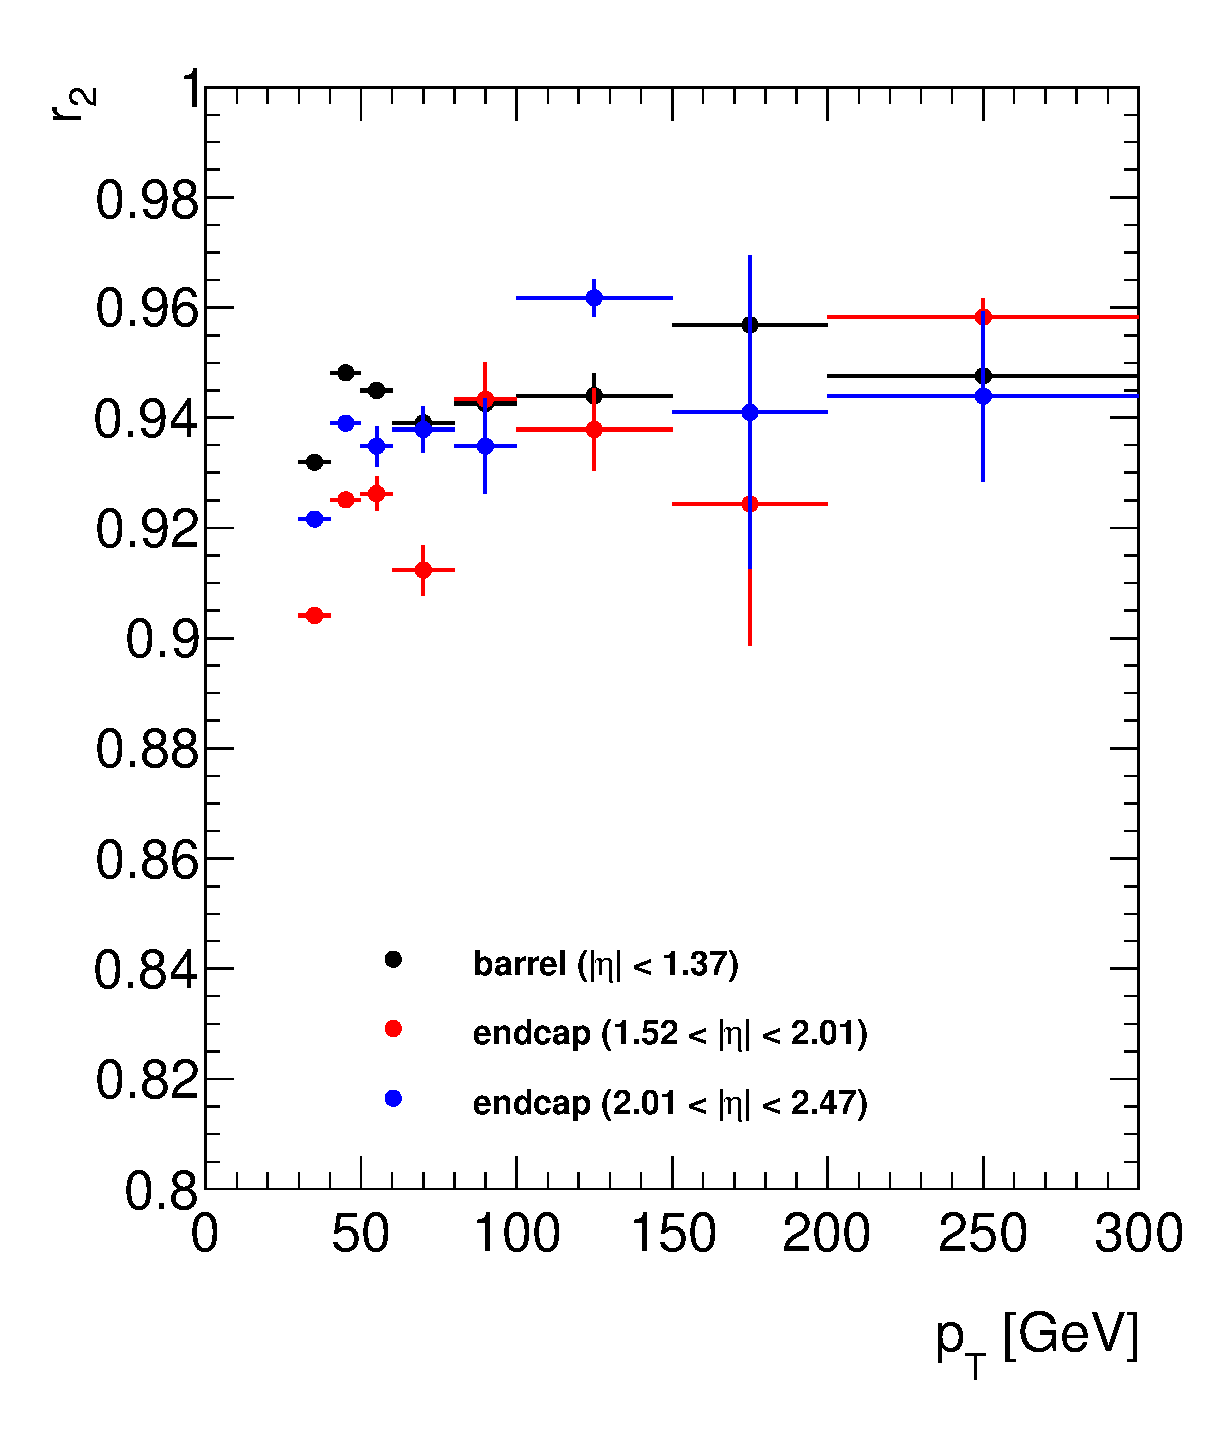
\includegraphics[scale=0.41]{images/r2.eps}
      \end{center}
   \caption{Real electron efficiencies obtained from Drell-Yan MC and binned in $p_{T}$ and three coarse $\eta$ bins covering the barrel and two endcap regions. Efficiencies for leading electrons are shown on the left while those for subleading electron are on the right.}
   \label{fig:realEff}
   \end{figure}



\subsection{Fake electron rate estimation}

The default method selected for analysing the fake rates is a single object method selection on the jet stream data. This gives the main advantage of more statistics and a higher energy reach compared to methods such as using tag and probe on the egamma stream data.
An array of triggers are used for selecting suitable events based on the single jet trigger EF\_jX\_a4chad (where X = 25, 35, 45, 55, 80, 110, 145, 180, 220, 280, 360). Events are associated to groups with the lowest trigger threshold they pass as each trigger has a different prescale. Objects are selected with the AntiKt4TopoEMJets algorithm and then matched to objects in the egamma stream with a $\Delta R~<~0.1$. Objects also have to pass the medium jet-cleaning criteria (define this). Two further steps are taken to suppress real electrons from W decays and real Drell-Yan events. A veto of $E_{Tmiss}~>~25~GeV$ is introduced to combat the former while events with two medium++ or loose++ electrons with $|m_{tag~\&~probe}-91~GeV|~<~20~GeV$ are vetoed to counter the real Drell-Yan.

The fake rate is then defined as Eq.~\ref{eq:fakeRate} $f~=~N^{fake}_{tight}/N^{fake}_{loose}$ with distributions selected using the standard event selection on the matched egamma objects.
Due to the different prescales of each trigger a separate set of fake rates are calculated for each trigger, these are then combined as a weighted average of all fake rates. Fig. \ref{fig:fakeRates} shows the distribution of fake rates for leading and subleading fakes which are distributed between 3 - $20\%$.

   \begin{figure}[h]
      \begin{center}
      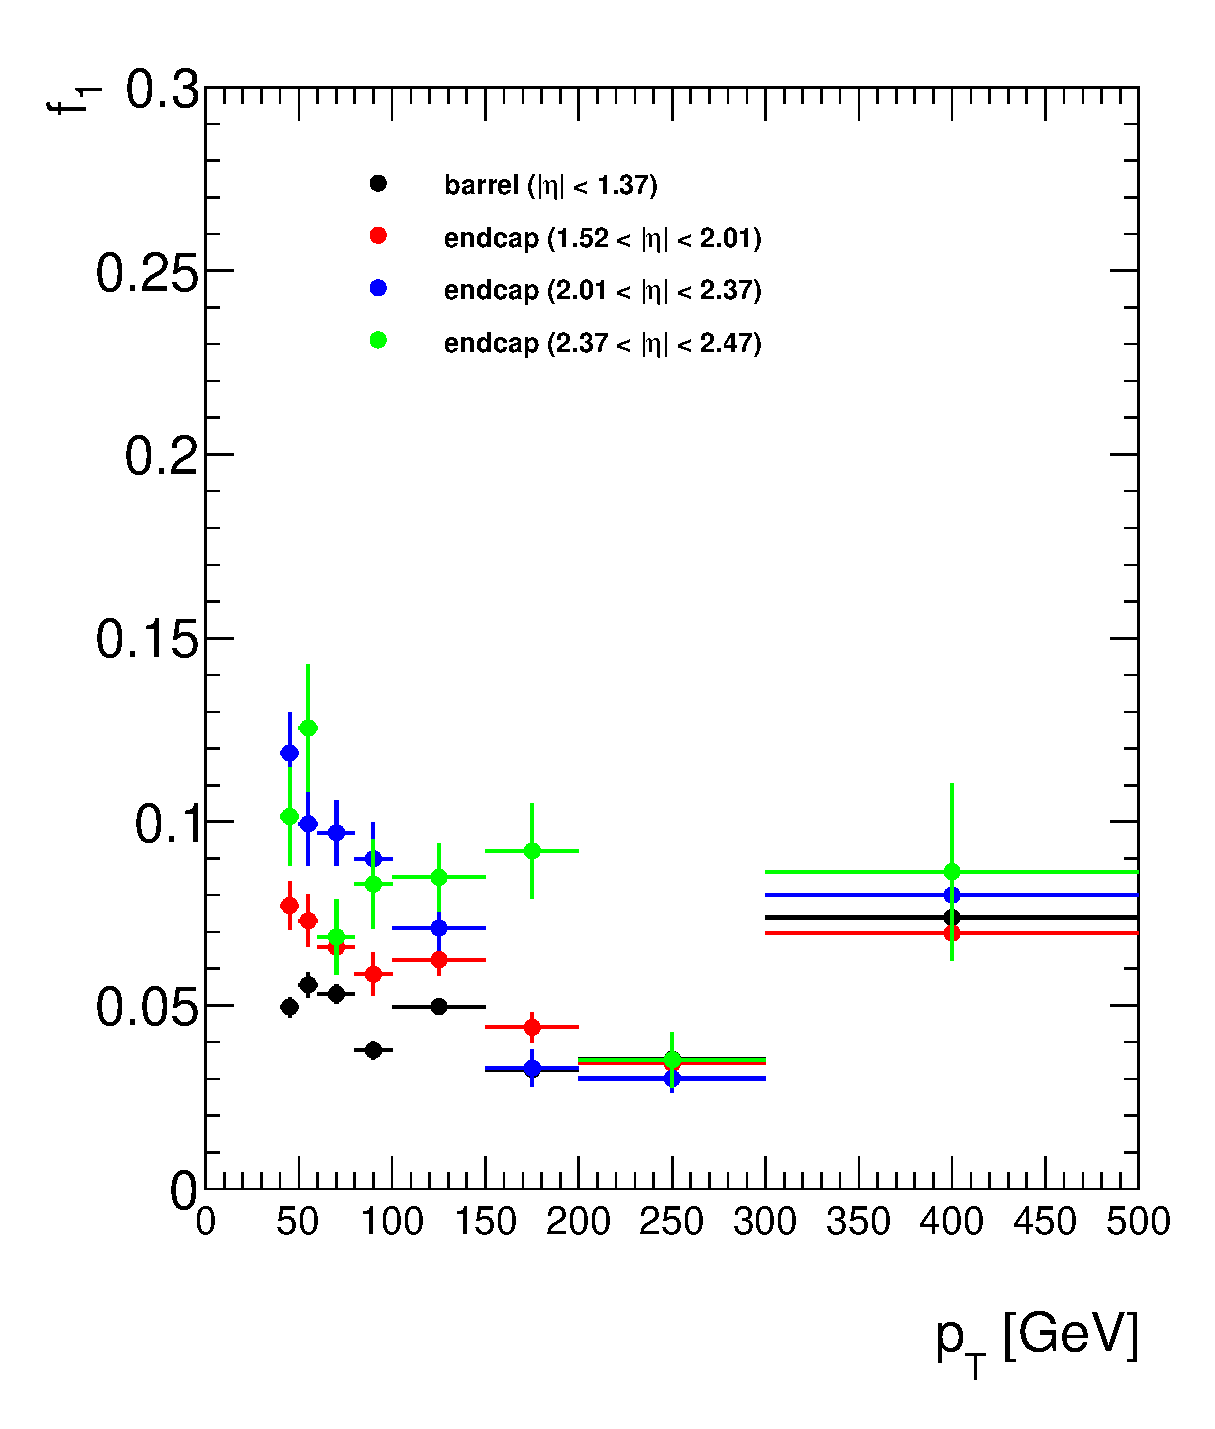
\includegraphics[scale=0.41]{images/f1.eps}
      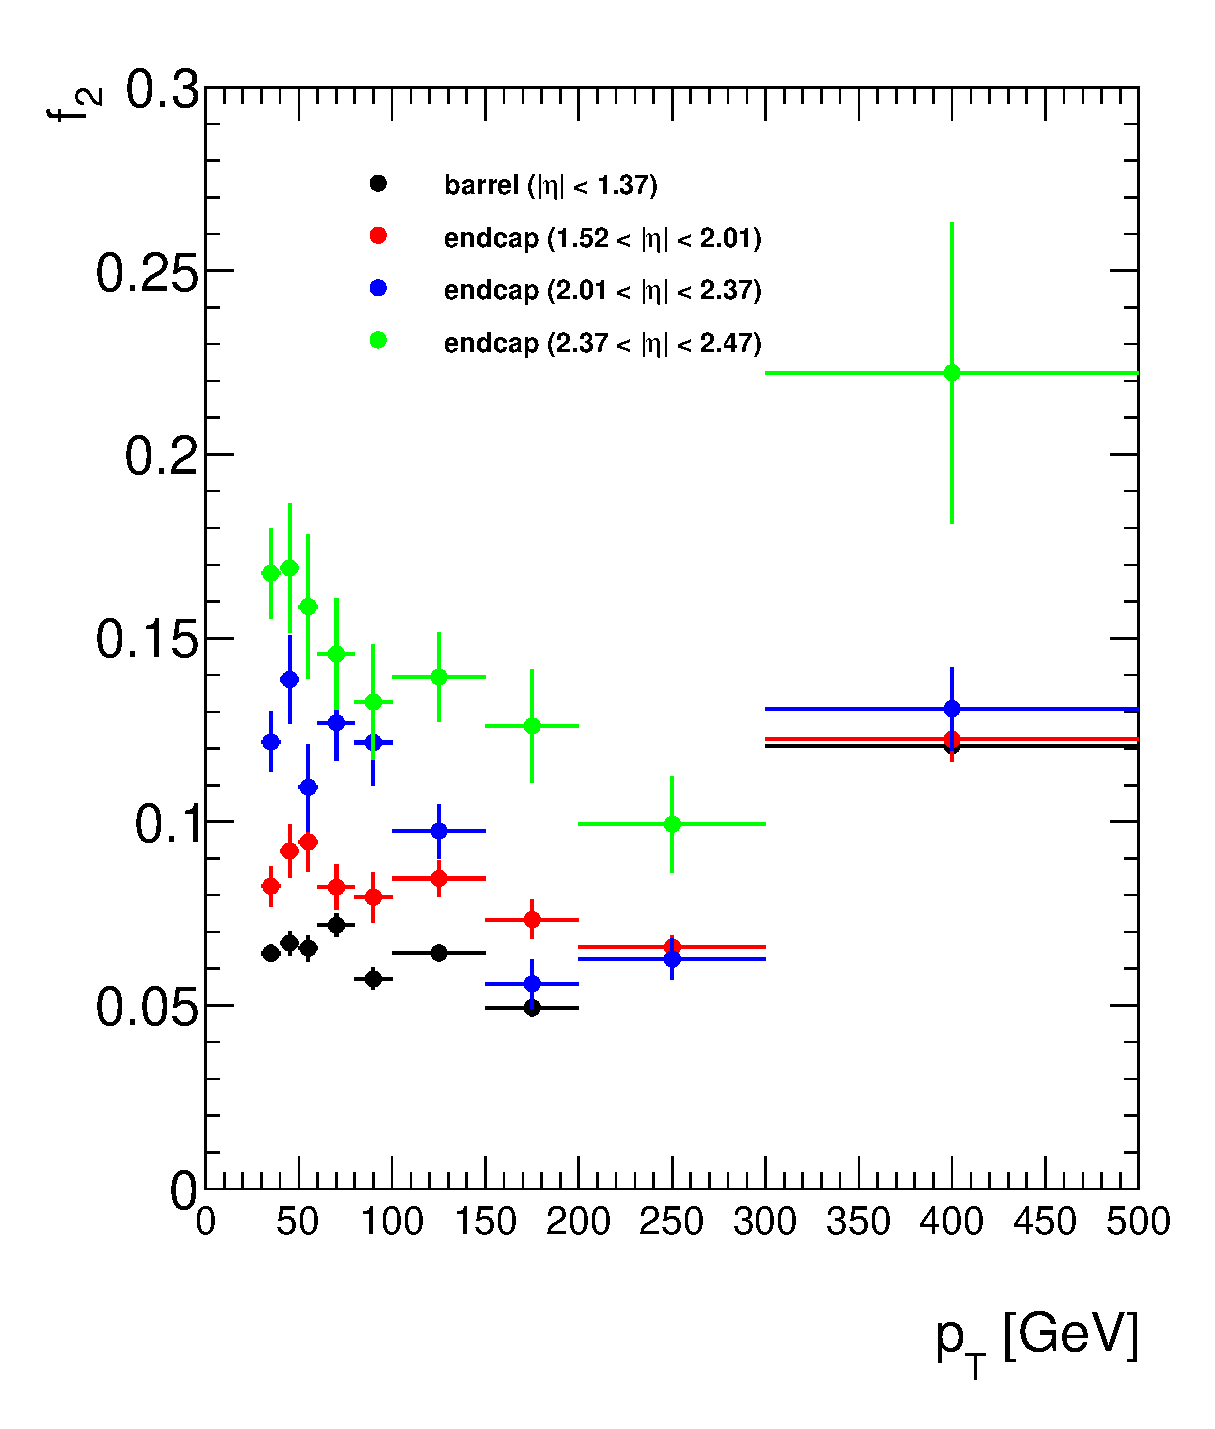
\includegraphics[scale=0.41]{images/f2.eps}
      \end{center}
   \caption{Fake rates obtained from data and binned in $p_{T}$ and four coarse $\eta$ bins covering the barrel and three endcap regions. Fake rates for leading electrons are shown on the left while those for subleading electron are on the right.}
   \label{fig:fakeRates}
   \end{figure}




\subsection{Properties of Multi-Jet Background}

In order to compose the final sample events are organised by the distributions $N_{TT}$, $N_{TL}$, $N_{LT}$ or $N_{LL}$ and weights are applied according to each electrons $p_{T}$, $\eta$ with respect to Eq.~\ref{eq:mainFakeResult} and the corresponding efficiencies and fake rates. 
Fig. \ref{fig:N_dist} shows these distributions before the efficiencies and fake rates are applied to weight to the final background prediction. In addition to these steps an extra fit is then applied at low invariant mass due to contamination due to the Z boson peak. This method is not suited to predicting the Multi-Jet background in the Z boson peak region and so a fit is obtained between 120 GeV and 400 GeV and stitched from 110 GeV and bellow. This gives a good estimate to the integral in this region for use in scaling MC's to luminosity but is not predicted to be good at predicting other variables in this region.

   \begin{figure}[h]
      \begin{center}
      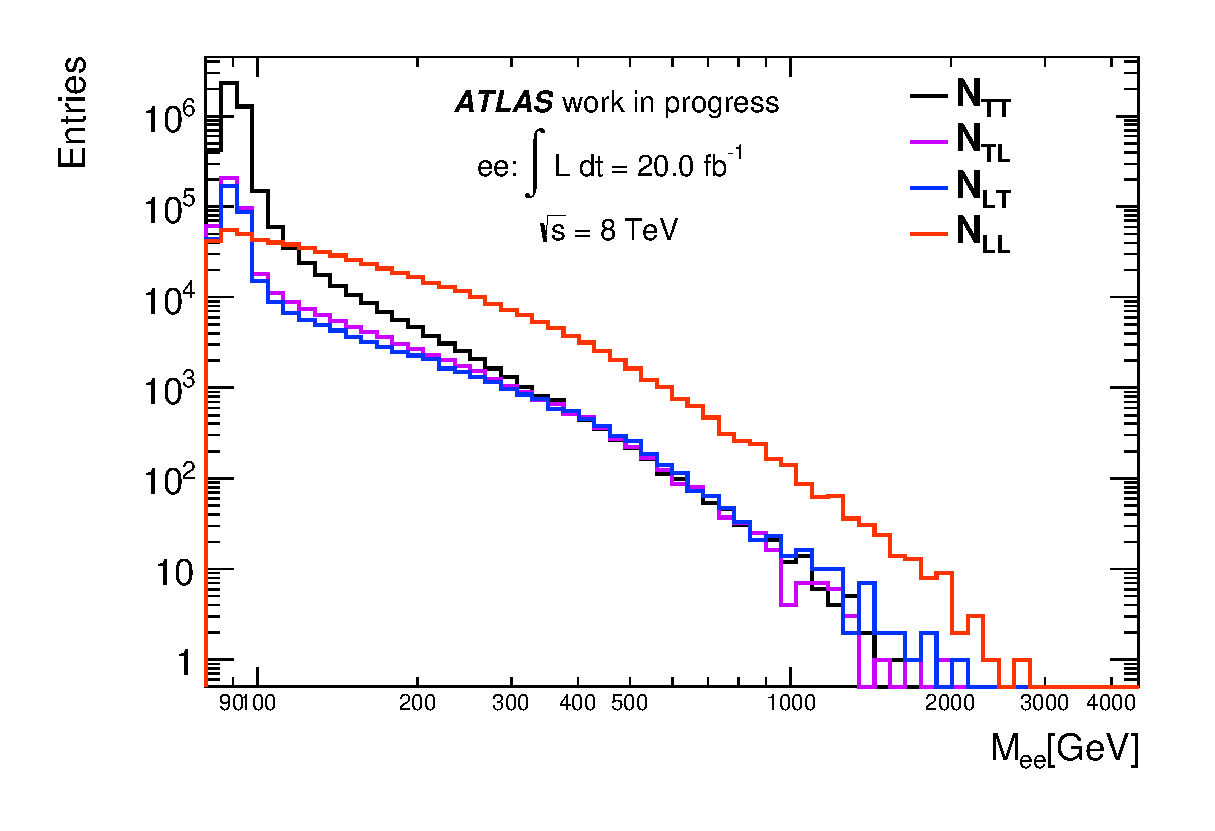
\includegraphics[scale=0.8]{images/N_distributions.eps}
      \end{center}
   \caption{Distribution of $N_{TT}$, $N_{TL}$, $N_{LT}$ and $N_{LL}$ from data with no weightings applied.}
   \label{fig:N_dist}
   \end{figure}






\subsection{Other methods and estimation of Error}


Two other methods and variations upon them were used to test the validity of this method as well as estimate the systematic error of this background estimates procedure. These two methods are both tag and probe measurements on either the jet stream of data, or the egamma stream where the method is more an "inverse" tag and probe with the selection of a tag with high probability of being a jet. Variations are also made on the method by assuming $r_{1}$ and $r_{2} = 1.0$ in all cases as well as changing the definition of loose but fail tight. These variations simplify the equations slightly but the method remains the same. Fig.~\ref{fig:ff_bkg_variation} shows all of these variations compared to the default method used to obtain the estimation. This figure then gives us a good estimate to the systematic uncertainty of the multi-jet estimate which has been chosen to be $20\%$. (ref zprime support note)

   \begin{figure}[h]
      \begin{center}
      \includegraphics[scale=1,trim={3cm 5.5cm 3cm 14cm},clip]{images/ff_bkg_variation.ps}
      \end{center}
   \caption{Ratio of the final background estimate of all method variations to the default method. The ratio starts at 116 GeV and ends at 1500 GeV. Source: resonant support note, will not be able to use this.}
   \label{fig:ff_bkg_variation}
   \end{figure}



\newpage




